\documentclass[12pt,a4paper]{article}
\usepackage[utf8]{inputenc}
\usepackage[T1]{fontenc}
\usepackage[french]{babel}
\usepackage{lmodern}
\usepackage{geometry}
\usepackage{graphicx}
\usepackage{float}
\geometry{margin=2.5cm}
\usepackage[colorlinks=true, linkcolor=purple]{hyperref}
\usepackage{listings}
\usepackage{xcolor}
\usepackage{booktabs}
\usepackage{colortbl}
\usepackage{pgfplots}
\pgfplotsset{compat=1.18}
\usepackage{tikz}
\usetikzlibrary{shapes.geometric,arrows.meta,positioning,calc,fit,backgrounds}
\definecolor{layerui}{RGB}{225,240,255}
\definecolor{layerlogic}{RGB}{235,225,255}
\definecolor{layerdata}{RGB}{220,245,235}
\definecolor{bordui}{RGB}{50,130,210}
\definecolor{bordlogic}{RGB}{100,60,190}
\definecolor{borddata}{RGB}{30,160,100}
\definecolor{coral}{RGB}{210,80,60}
 
\tikzset{
  module/.style={rectangle, rounded corners=5pt, minimum width=2.2cm, minimum height=0.8cm,
    font=\small\bfseries, text centered, inner sep=4pt},
  uimod/.style={module, fill=layerui, draw=bordui, text=bordui},
  logmod/.style={module, fill=layerlogic, draw=bordlogic, text=bordlogic},
  datamod/.style={module, fill=layerdata, draw=borddata, text=borddata},
  coralmod/.style={module, fill={rgb,255:red,255;green,235;blue,230}, draw=coral, text=coral},
  layerbg/.style={rectangle, rounded corners=8pt, draw, dashed, inner sep=10pt, opacity=0.6},
  arr/.style={-{Stealth[length=5pt]}, thick, opacity=0.55},
  darr/.style={-{Stealth[length=5pt]}, thick, opacity=0.4, dashed},
  layerlabel/.style={font=\footnotesize\itshape, opacity=0.6}
}
\usepackage{caption}
\usepackage{subcaption}
\usepackage{array}
\usepackage{verbatim}
\usepackage{amsmath}

\definecolor{okgreen}{RGB}{29,158,117}
\definecolor{warncolor}{RGB}{186,117,23}
\definecolor{errcolor}{RGB}{226,75,74}
\definecolor{codebg}{RGB}{245,245,245}
\definecolor{codeframe}{RGB}{180,180,180}

\lstset{
  language=Java,
  basicstyle=\ttfamily\small,
  backgroundcolor=\color{codebg},
  frame=single,
  rulecolor=\color{codeframe},
  breaklines=true,
  numbers=left,
  numberstyle=\tiny\color{gray},
  keywordstyle=\color{blue}\bfseries,
  commentstyle=\color{gray}\itshape,
  stringstyle=\color{red},
  showstringspaces=false,
  captionpos=b,
  literate={é}{{\'{e}}}1 {è}{{\`{e}}}1 {à}{{\`{a}}}1
}

\begin{document}

\begin{titlepage}

  \begin{flushleft}
    
\includegraphics{images/Logo_ENSEIRB.png}
  \end{flushleft}

  \vspace*{\fill}

  \begin{center}
    {\Huge \textbf{Rapport de Projet : Robot Programming}}\\[0.5cm]
    {\large Variante de Robozzle}\\[2cm]

    {\LARGE
      Wassim LQADI, Jessim AZZAG, Yoann ETHE, Rayane AOUSSAR
      }\\[2cm]

    {\large Mai 2026}

  \end{center}
  \vspace*{\fill}

\end{titlepage}

\tableofcontents
\newpage

% ============================================================
\section{Introduction et contexte}
% ============================================================

Le projet \textit{Robozzle} consiste à concevoir un solveur de puzzles logiques. L'approche privilégie le typage statique fort et l'immutabilité des données.

Le projet Robot Programming demande de concevoir un moteur d'exécution capable de faire naviguer un robot sur une grille, en interprétant un programme fourni sous forme de pile d'instructions. 
Développé en TypeScript, le projet impose d'explorer les concepts de la programmation fonctionnelle (immutabilité, pureté, récursivité) au sein d'un environnement web.

% ============================================================
\section{Modélisation et typage}
% ============================================================

Chaque élément du jeu (Robot, Grille, Instructions, etc...) est défini par un type TypeScript strict. Cela permet d'éliminer de nombreuses erreurs de logique dès la compilation.

Contrairement à la programmation en C où les données sont de simples entiers non typés, TypeScript nous permet de définir des Types Abstraits de Données structurés et stricts.

\begin{lstlisting}[language=Java, basicstyle=\ttfamily\small, frame=single]
type Direction = 0 | 1 | 2 | 3;
type Robot = { col: number; row: number; dir: Direction; };
\end{lstlisting}

\begin{figure}[h!]
  \centering
  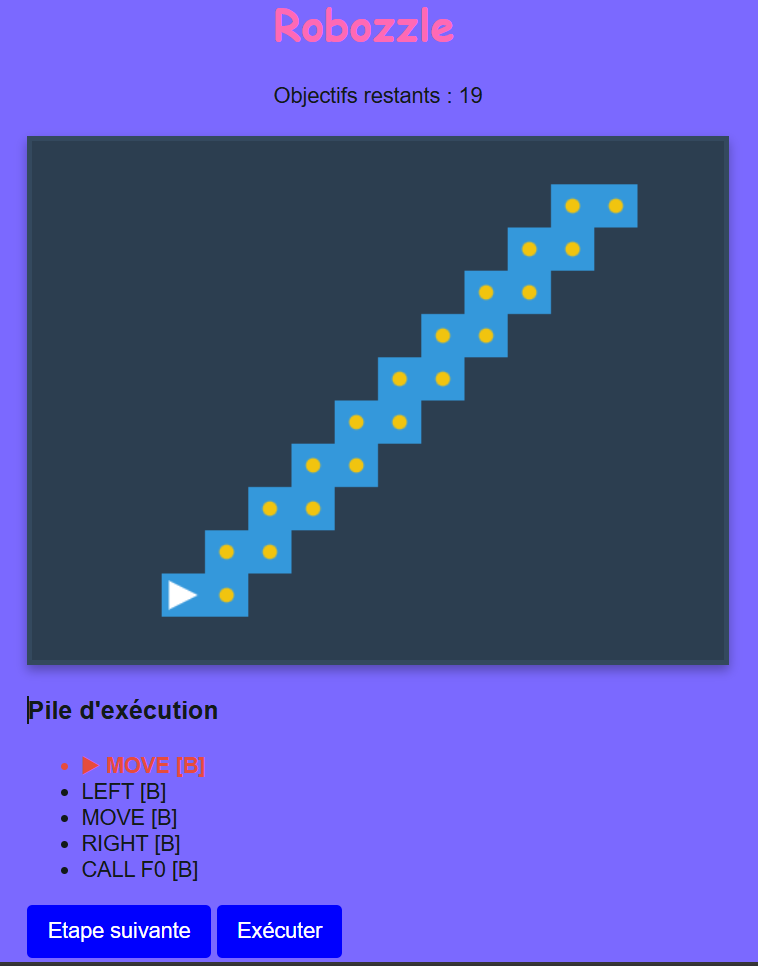
\includegraphics[width=0.6\textwidth]{images/rendu_projet.png} 
  \caption{Visualisation de l'état du robot et de la grille via l'interface du projet.}
  \label{fig:rendu_global}
\end{figure}

La Figure~\ref{fig:rendu_global} permet de visualiser la concrétisation de ces types : 
le \texttt{Robot} est ici positionné aux coordonnées calculées par sa structure, tandis que son orientation graphique traduit directement la valeur de l'union littérale \texttt{Direction}. 
Ce rendu met en évidence la correspondance entre l'état interne immuable de la simulation et sa traduction visuelle sur l'interface utilisateur, validant ainsi la cohérence de notre modèle de données.

\bigskip

\textbf{Justification :} Le système de types agit comme un protocole de validation statique (lors de la compilation via \texttt{tsc}). 
En définissant \texttt{Direction} comme une union littérale stricte, nous interdisons au compilateur d'accepter toute autre valeur numérique. 
Lors de l'implémentation des rotations (\texttt{RIGHT=0, SOUTH=1, EAST=2, WEST=3}) du \texttt{Robot}, le typage nous a forcés à prouver au compilateur (via un \textit{cast}) que l'invariant était respecté, 
éliminant ainsi toute une classe de bugs d'exécution.

\section{Architecture du projet}


Réfléchir à ce projet en modules était important, le projet nécessite d'implémenter beaucoup d'éléments différents et les implémenter tous au sein d'un seul fichier n'était pas une idée réaliste du tout. Il a fallu réfléchir à comment segmenter le travail pour éviter les bugs qui freinent l'ensemble de l'avancée.


\subsection{Découpage en modules}

En se basant sur nos imports notre projet peut être découpé en 4 couches. On a une première couche \texttt{World} qui comprend les fichiers \textit{world.ts et puzzle.ts}, ces fichiers définissent tous les types nécessaires (\texttt{Puzzle, Cell, Robot et World}) ainsi que les objectifs présents sur le monde. Ces deux fichiers constituent le socle du projet définissant l'ensemble des outils dont on a besoin pour réaliser le projet. 
\bigskip
Ensuite on a une autre couche qui se concentre sur \texttt{la pile de jeu}. L'un des aspects les plus importants du projet est la mise en place d'une \texttt{pile de jeu} comprenant des instructions et des fonctions ainsi que \texttt{la mise en relation} de ces dites instructions et du monde. Cette couche est donc multifonctionnelle, elle gère aussi bien les actions du robot que les conditions et les réponses de ces dites actions par rapport au monde. 

\begin{figure}[H]
    \centering
    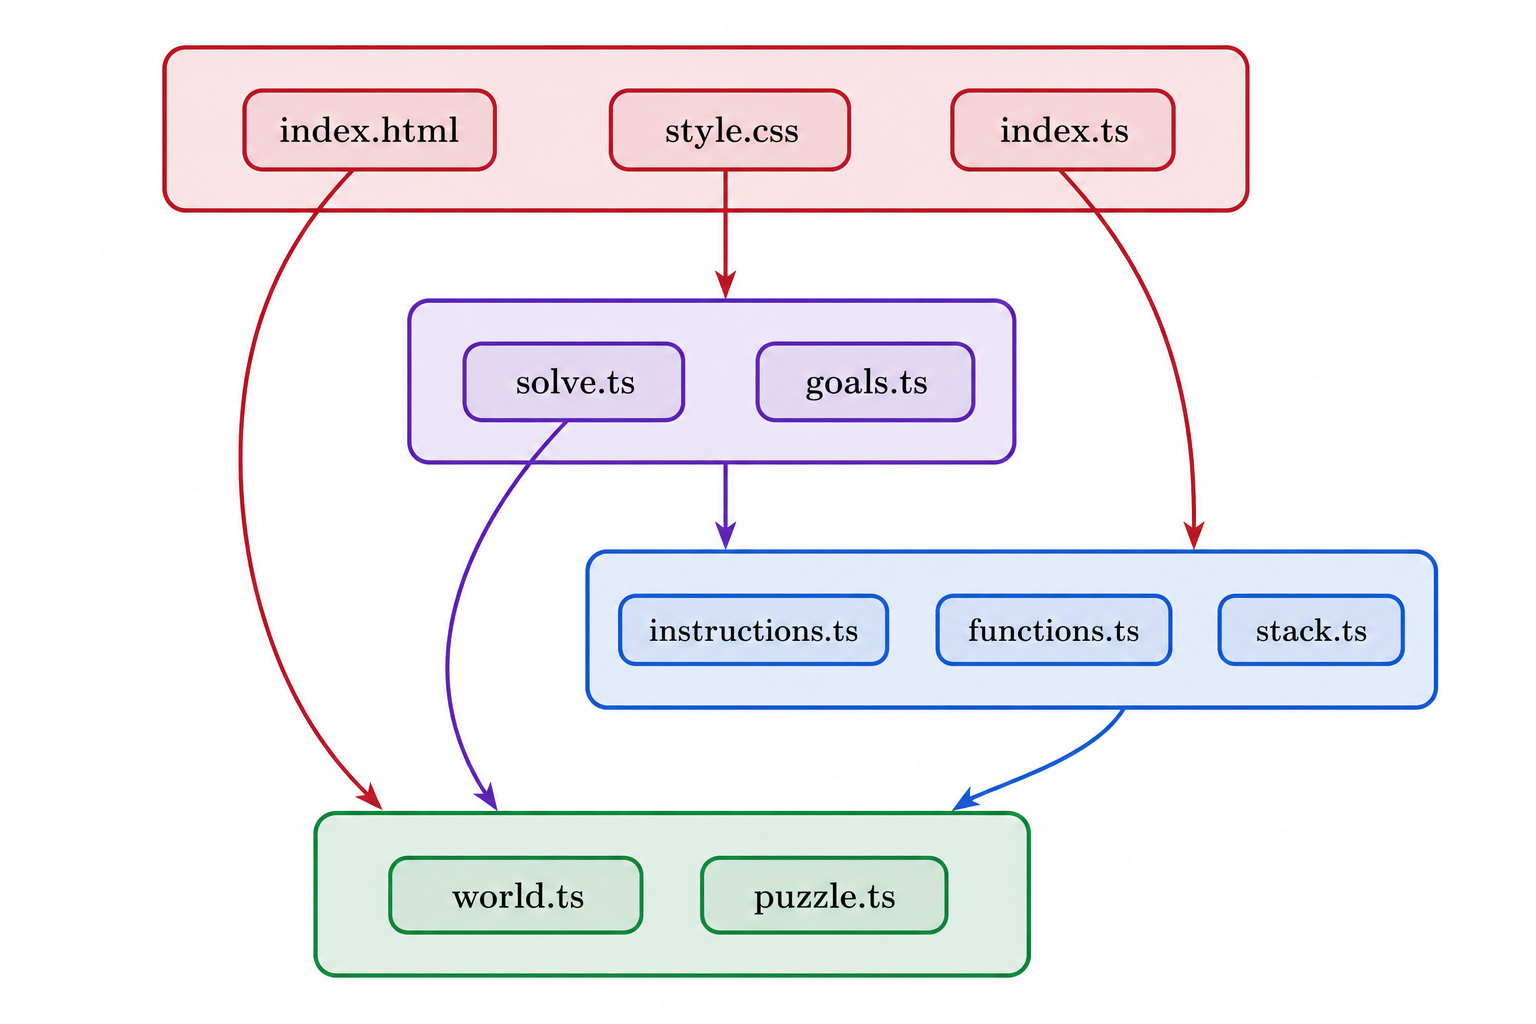
\includegraphics[width=0.8\textwidth]{images/image_arch.png}
    \caption{Graphe des dépendances}
    \label{fig:architecture}
\end{figure}

Enfin vient une couche composée de deux fichiers \textit{solve.ts et goals.ts} dans la Figure~\ref{fig:architecture}. cette couche gère la conception d'une solution à un puzzle donné.
 le fichier \textit{goals.ts} s'occupe de faire le décompte des objectifs pendant que \textit{solve.ts} gère la résolution du puzzle. Ce dernier vérifie qu'une pile donnée résout bien le puzzle. 
 Ainsi cette couche doit faire appel aux deux autres couches car elle demande \texttt{la conception d'une pile pour résoudre un monde}.

La dernière couche s'occupe de l'affichage, on y retrouve les fichiers \textit{index.ts, index.html et style.css}. Cela met en lumière \textit{la multidépendance} de toutes les couches fonctionnelles.

\subsection{Pile d'exécution}

Une particularité de notre architecture est que les fichiers établissant notre pile d'appel \textit{instructions.ts, function.ts et stack.ts} s'incluent mutuellement, ce qui fait des inclusions circulaires. 
Toutefois la particularité fonctionnelle du projet permet d'importer uniquement les fonctions dont on a besoin se mettant ainsi à l'abri des inclusions circulaires en tant que tel.

\begin{figure}[H]
    \centering
    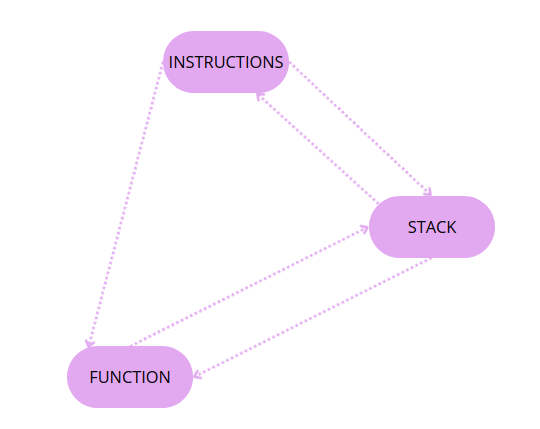
\includegraphics[width=0.5\textwidth]{images/img1.png}
    \caption{Dépendances circulaires au sein du module pile}
    \label{fig:architecture2}
\end{figure}


% ============================================================
\section{Architecture logicielle : immutabilité et simulation}
% ============================================================

Dans un paradigme impératif, nous aurions modifié le tableau à deux dimensions directement (\texttt{world.cells[y][x].hasStar = false}). 
Ici, la démarche fonctionnelle nous a poussés à opter pour une approche pure.

\begin{lstlisting}[language=Java, basicstyle=\ttfamily\small, frame=single, title={Extrait de la logique d'immutabilité}]
function collectStar(world: World, row: number, col: number): World {
   const newCells = world.cells.map((r, ri) =>
     r.map((cell, ci) =>
       ri === row && ci === col ? { ...cell, hasStar: false } : cell
     )
   );
   return { ...world, cells: newCells };
}
\end{lstlisting}

\textbf{Analyse de la démarche :} La fonction \texttt{collectStar} prend un état $E$ et retourne un nouvel état $E'$. 
Elle utilise l'opérateur de décomposition et la fonction d'ordre supérieur \texttt{map}. 
Bien que cela génère des allocations mémoire supplémentaires à chaque étape, cette immutabilité garantit l'absence d'effets de bord. 
Le composant graphique de rendu du jeu devient totalement indépendant de la logique métier, facilitant la séparation des préoccupations.

\subsection{Le simulateur, la pile et la récursivité}

L'exécution des programmes repose sur une gestion LIFO (Last In, First Out). La structure du code évite les décompositions trop fines pour maintenir une vision d'ensemble cohérente.

L'exécution du programme du robot s'appuie fortement sur le concept de pile (\texttt{Stack}). Lorsqu'une instruction de type \texttt{CALL} est rencontrée, 
le robot doit suspendre son exécution courante et insérer le code d'une nouvelle fonction.

Nous avons traité ce problème en manipulant notre type \texttt{Stack} de manière non-destructrice : \texttt{myStack = [...newInstructions, ...myStack]}. 
Ce choix fait écho aux structures de données récursives. L'exécution d'une instruction (fonction \texttt{execInstruct}) s'appelle elle-même jusqu'à ce que la condition d'arrêt (pile vide ou objectif atteint) soit vérifiée. 
Cette formulation est beaucoup plus proche des définitions formelles mathématiques qu'une boucle \texttt{while} impérative.

\subsection{Optimisation et robustesse via le paradigme fonctionnel}

Bien que l'architecture initiale réponde aux exigences, son évolution et sa maintenabilité reposent sur l'adoption stricte des concepts avancés de la programmation fonctionnelle. 
Cette sous-partie détaille comment ces principes optimisent et sécurisent la logique métier.

\subsubsection*{Les fonctions comme citoyennes de première classe}
En TypeScript, les fonctions sont traitées comme des \textit{citoyennes de première classe} : 
elles peuvent être assignées, retournées ou passées en argument. 
Dans la gestion des actions du robot, passer l'action spécifique (le \textit{callback}) à une fonction de vérification d'état (comme \texttt{executeIfColorMatches}) permet de factoriser la logique conditionnelle. 
Cela évite la duplication du code pour les instructions \texttt{MOVE}, \texttt{LEFT}, \texttt{RIGHT} ou \texttt{CALL}, 
rendant l'architecture hautement modulaire.

\subsubsection*{Pureté et élimination des effets de bord}
Une approche impérative classique impliquerait des mutations directes sur l'objet \texttt{Robot} (par exemple, \texttt{robot.col += dc}). 
Ces \textbf{effets de bord} rendent l'état du système imprévisible et le débogage complexe. 
L'optimisation fonctionnelle exige au contraire des \textbf{fonctions pures} : 
pour les mêmes arguments, elles retournent un nouveau résultat sans jamais altérer d'état externe.

\begin{lstlisting}[language=Java, basicstyle=\ttfamily\small, frame=single, title={Exemple d'approche pure pour le déplacement}]
const actions = {
  MOVE: (robot: Robot) => {
    const mods = [[1, 0], [0, 1], [-1, 0], [0, -1]];
    const [dc, dr] = mods[robot.dir % 4];
    return { ...robot, col: robot.col + dc, row: robot.row + dr };
  }
};
\end{lstlisting}

Cette pureté garantit la prédictibilité totale du code et simplifie drastiquement l'écriture des tests unitaires (cf. Section \ref{sec:tests}), 
puisqu'il n'est plus nécessaire de réinitialiser l'état entre chaque test.

\subsubsection*{Persistance et immutabilité}
Le corollaire de la pureté est l'immutabilité des structures de données. 
En générant de nouveaux états (via l'opérateur de décomposition \texttt{...}) plutôt qu'en écrasant les anciens, 
nous créons des structures de données \textbf{persistantes}. 
Dans le contexte d'un jeu ou d'un solveur de puzzle, cette persistance offre un avantage majeur : 
elle permet de conserver nativement l'historique complet des états du robot. 
Implémenter une fonctionnalité de \textit{Retour en arrière} ou tracer l'historique d'exécution pas-à-pas devient trivial, 
car l'historique n'est qu'un simple tableau d'états immuables successifs.

\subsubsection*{Modélisation via les types inductifs}
Plutôt que d'utiliser des dictionnaires d'actions isolés, le style fonctionnel s'appuie sur les \textbf{types inductifs}, 
traduits en TypeScript par des unions discriminées. 

\begin{lstlisting}[language=Java, basicstyle=\ttfamily\small, frame=single, title={Modélisation par types inductifs}]
type Instruction = 
  | { type: 'MOVE' }
  | { type: 'TURN', direction: 'LEFT' | 'RIGHT' }
  | { type: 'CALL', functionId: number };
\end{lstlisting}

Couplée à une fonction d'évaluation (un \textit{reduce}), 
cette modélisation offre une sécurité absolue à la compilation. 
Par exemple, si une nouvelle instruction venait à être ajoutée au jeu (ex: \texttt{JUMP}), 
TypeScript signalerait immédiatement toutes les zones du code où cette instruction n'est pas traitée, 
éliminant ainsi les angles morts de la logique d'exécution.

% ============================================================
\section{Génération de mondes et résolution automatique de puzzles}

Cette section présente les approches envisagées pour deux fonctionnalités que le temps de développement n'a pas permis d'implémenter : la génération procédurale de mondes valides, et la résolution automatique de puzzles par exploration de l'espace des programmes. Nous en proposons une formalisation, une analyse de complexité et une discussion sur leur adéquation à l'aspect fonctionnel du projet.

\subsection{Génération de mondes}

\subsubsection*{Définition formelle du problème}

Un monde valide doit satisfaire les contraintes suivantes :
\begin{itemize}
  \item La grille est de taille $12 \times 16 = 192$ cases.
  \item Chaque case appartient à $\{\texttt{B}, \texttt{R}, \texttt{G}, \texttt{N}\}$, la couleur \texttt{N} étant inaccessible.
  \item Le robot est positionné sur une case accessible (non \texttt{N}).
  \item Au moins une étoile est placée sur une case accessible, et l'ensemble des cases étoilées est atteignable depuis la position initiale du robot.
\end{itemize}

La condition d'atteignabilité est la contrainte la plus importante pour pouvoir implémenter un solveur : sans elle, on génère des puzzles insolubles par construction.

\subsubsection*{Génération aléatoire naïve}

L'approche la plus simple consiste à tirer chaque case uniformément dans $\{\texttt{B}, \texttt{R}, \texttt{G}, \texttt{N}\}$, à placer le robot sur une case accessible choisie au hasard, puis à rejeter tout monde ne satisfaisant pas la condition d'atteignabilité (en testant à chaque fois).

\subparagraph{Complexité.}
Soit $n = 192$ le nombre de cases. La vérification d'atteignabilité s'effectue par un BFS/DFS depuis la position initiale du robot, en $\mathcal{O}(n)$. La probabilité qu'un tirage aléatoire produise une composante connexe suffisante dépend de la densité de cases accessibles, donc de la probabilité qu'une case ne soit pas \texttt{N} qui est ${3/4}$ dans notre cas. La probabilité de rejeter un monde est donc faible, mais le nombre de tentatives avant succès est en $\mathcal{O}(1)$ en espérance puisque la probabilité $p$ qu'un monde soit valide est constante, ce qui veut dire que l'espérance de la variable aléatoire $T$, représentant le nombre de tentatives avant succès, qui est ~$E[T]=1/p$~ est également constante. La complexité globale est donc $\mathcal{O}(n)$ en moyenne.

\subparagraph{Limite.}
Cette approche génère des mondes structurellement faibles : les cases colorées sont réparties aléatoirement, sans logique de puzzle. Le programme résolvant un tel monde est généralement trivial (boucle MOVE-CALL) ou inexistant.

\subsubsection*{Génération guidée par le programme}

Une meilleure approche consiste à inverser la démarche :
\begin{enumerate}
  \item Tirer aléatoirement un programme $P$ valide (respectant les contraintes de taille).
  \item Simuler l'exécution de $P$ depuis une position initiale pour tracer le chemin parcouru.
  \item Construire le monde en coloriant les cases du chemin et en y plaçant des étoiles.
\end{enumerate}

Cette technique garantit par construction qu'il existe au moins un programme résolvant le puzzle généré.

\subparagraph{Complexité.}
Soit $I$ le nombre maximal d'instructions autorisées ($I = 1000$ dans notre cas). La simulation de $P$ s'effectue en $\mathcal{O}(I)$. La construction du monde à partir du chemin est en $\mathcal{O}(n)$. La complexité totale est $\mathcal{O}(I + n) = \mathcal{O}(I)$ puisque $I \gg n$ en pratique.

\subsection{Résolution automatique : solveurs}

Résoudre un puzzle revient à trouver un programme $P$ dans l'espace $\mathcal{P}$ de tous les programmes valides (respectant les contraintes du puzzle) tel que l'exécution de $P$ sur le monde $W$ atteint l'objectif $G$.

\subsubsection*{Taille de l'espace de recherche}

Soit $F$ le nombre de fonctions, $S_i$ la taille maximale de la fonction $i$, $C$ le nombre d'instructions disponibles et $K = 4$ le nombre de couleurs de condition (B, R, G, N). Chaque slot d'instruction peut accueillir $C \times K$ valeurs ou être vide. Le nombre total de programmes est :

\[
  |\mathcal{P}| = \prod_{i=1}^{F} (C \cdot K + 1)^{S_i}
\]

En l'occurrence, pour le cas typique $F = 5$, $S_i = 10$, $C = 4$ instructions de base, $K = 4$ :

\[
  |\mathcal{P}| \approx 10^{61}
\]

Cet espace est beaucoup trop grand pour une exploration exhaustive, d'où l'intérêt des heuristiques.

\subsubsection*{Recherche par A*}

\subparagraph{Modélisation.}
On modélise la recherche comme un problème de plus court chemin dans un graphe d'états. Un état est un triplet $(monde, robot, pile)$, et chaque transition correspond à l'exécution d'une instruction. L'algorithme A* sélectionne à chaque étape l'état minimisant $f(s) = g(s) + h(s)$, où $g(s)$ est le coût depuis l'état initial (nombre d'instructions exécutées) et $h(s)$ une heuristique admissible.

\subparagraph{Heuristique.}
Une heuristique naturelle est la \textbf{distance de Manhattan} entre le robot et l'étoile la plus proche. En notant $\mathcal{E}$ l'ensemble des cases encore étoilées :

\[
  h(s) = \min_{(r,c)\,\in\,\mathcal{E}} \bigl(|r - r_{\mathrm{robot}}| + |c - c_{\mathrm{robot}}|\bigr)
\]

Cette heuristique est admissible car le robot avance d'au plus une case par instruction MOVE, et ne peut donc atteindre une étoile en moins de $h(s)$ pas.

\subparagraph{Complexité.}
Dans le pire cas, A* explore un nombre d'états exponentiel en la profondeur de la solution. Avec une heuristique efficace, la complexité pratique est $\mathcal{O}(m^{d/2})$ où $m$ est le nombre moyen de successeurs possibles depuis un état (ici $m = C \cdot K = 16$) et $d$ la profondeur optimale. La mémoire requise est également $\mathcal{O}(m^{d/2})$, ce qui constitue un véritable problème pour les puzzles profonds.

\subparagraph{Limite.}
A* est optimal pour trouver le \textit{programme le plus court}, mais reste inadapté aux puzzles dont la solution requiert de nombreuses instructions imbriquées, car la complexité devient exponentielle. De plus, la modélisation de l'espace d'états doit intégrer la pile d'appel pour ne pas confondre des états différents, ce qui augmente considérablement la dimension de l'espace.

\subsubsection*{Algorithmes génétiques}

\paragraph{Principe.}
Les algorithmes génétiques maintiennent une \textit{population} de programmes candidats, qu'ils font évoluer par \textit{sélection}, \textit{croisement} et \textit{mutation} au fil de générations successives.

\begin{enumerate}
  \item \textbf{Encodage.} Un programme est encodé comme une chaîne de caractères : chaque instruction est représentée par un couple (type, couleur), les fonctions étant séparées par un délimiteur. Deux programmes peuvent ainsi être \textit{croisés} en échangeant des segments de leurs chaînes respectives.
  \item \textbf{Fonction de fitness.} On évalue chaque programme en le simulant et en comptant le nombre d'étoiles collectées et en retranchant des points $\alpha$ pour les erreurs d'exécution (\textit{Out of ground}, \textit{Infinite loop}).
        \[
          \text{fitness}(P) = \text{étoiles collectées}(P) - \alpha \cdot \mathbf{1}[\text{erreur}(P)]
        \]
  \item \textbf{Sélection.} Les programmes de meilleur fitness sont sélectionnés préférentiellement pour la reproduction (par tournoi).
  \item \textbf{Croisement.} Deux programmes $P_1, P_2$ échangent une sous-séquence d'instructions pour produire deux fils.
  \item \textbf{Mutation.} Une instruction d'un programme est remplacée aléatoirement avec une faible probabilité $p_m$ (typiquement $p_m$ de l'ordre de $10^{-2}$).
\end{enumerate}

\paragraph{Complexité.}
Soit $N$ la taille de la population, $G$ le nombre de générations et $I$ le coût de simulation d'un programme. La complexité par génération est $\mathcal{O}(N \cdot I)$, et la complexité totale est $\mathcal{O}(G \cdot N \cdot I)$. Si $N = 200$, $G = 1000$ et $I = \mathcal{O}(1000)$ instructions, on obtient $\mathcal{O}(2 \times 10^8)$ opérations élémentaires, ce qui est raisonnable en quelques secondes sur une machine moderne.

\paragraph{Aspect fonctionnel.}
La génération d'une population et son évolution s'expriment naturellement
comme des transformations sur des listes immuables :

\begin{verbatim}
const nextGeneration = (population: program[]): program[] =>
  Array.from({ length: population.length }, () =>
    mutate(crossover(select(population), select(population)))
  );
\end{verbatim}

Chaque génération est produite par application de fonctions pures, sans état global mutable, ce qui est cohérent avec l'aspect fonctionnel du projet.

\paragraph{Limite.}
La convergence prématurée vers un optimum local est le principal inconvénient des algorithmes génétiques. Des techniques de maintien de la diversité peuvent être envisageables.

\subsubsection*{Comparaison des approches}

\begin{table}[h]
\centering
\begin{tabular}{|l|c|c|c|c|}
\hline
\textbf{Algorithme} & \textbf{Optimal} & \textbf{Complet} & \textbf{Complexité temps} & \textbf{Complexité mémoire} \\
\hline
Exhaustif & Oui & Oui & $\mathcal{O}(|\mathcal{P}|)$ & $\mathcal{O}(|\mathcal{P}|)$ \\
A* & Oui & Oui & $\mathcal{O}(m^{d/2})$ & $\mathcal{O}(m^{d/2})$ \\
Génétique & Non & Non & $\mathcal{O}(G \cdot N \cdot I)$ & $\mathcal{O}(N \cdot I)$ \\
\hline
\end{tabular}
\caption{Comparaison des stratégies de résolution. $m$ : nombre moyen de successeurs depuis un état, $d$ : profondeur optimale, $G$ : générations, $N$ : taille de population, $I$ : coût de simulation.}
\end{table}

En pratique, l'algorithme génétique constitue le meilleur compromis pour les puzzles de grande taille : il ne garantit pas de trouver la solution optimale, mais converge vers une solution acceptable en temps polynomial. A* reste préférable pour les puzzles de petite taille, où son optimalité est exploitable.

\subsection{Bilan}

Les deux fonctionnalités présentées ici, la génération de mondes et la résolution automatique, constituent des extensions du simulateur de programmes développé. Leur formalisation met en évidence plusieurs points importants :

\begin{itemize}
  \item La génération guidée par le programme est la seule approche pour produire des puzzles \textit{bien pensés}.
  \item La taille de l'espace de recherche ($\approx 10^{61}$ programmes dans le cas général) rend l'exploration exhaustive inenvisageable ; des heuristiques sont indispensables.
  \item Les deux algorithmes de résolution s'intègrent naturellement au paradigme fonctionnel :
  \item Le coût prépondérant dans tous ces algorithmes est la simulation ($\mathcal{O}(I) = \mathcal{O}(1000)$ par programme), ce qui justifie le besoin de maximiser le nombre d'évaluations parallèles dans une implémentation réelle.
\end{itemize}

% ============================================================

% ============================================================
\section{Tests et validation}
\label{sec:tests}
% ============================================================

Le protocole de test du projet Robozzle repose sur la même démarche
scientifique que pour Coursidor~: chaque test traduit une
\emph{spécification fonctionnelle} en \emph{assertion vérifiable
automatiquement}. L'outillage diffère — Jest, ts-jest et Istanbul
en TypeScript contre \texttt{assert} et \texttt{gcov} en C — mais la
logique est identique. TypeScript apporte de surcroît une couche de
validation \emph{statique} avant l'exécution~: le compilateur rejette
un appel mal typé avant même que les tests ne soient lancés.

Cette section présente l'organisation des tests
(\S\ref{subsec:r-orga}), les résultats de couverture obtenus avec
Jest~--~Istanbul (\S\ref{subsec:r-coverage}), les bugs détectés et
corrigés (\S\ref{subsec:r-bugs}), puis les limites et pistes
d'amélioration (\S\ref{subsec:r-limites}).

\subsection{Organisation des tests}
\label{subsec:r-orga}
 
Les 43 tests sont répartis en six fichiers, chacun ciblant un module
précis du projet.
 
\begin{table}[h!]
\centering
\renewcommand{\arraystretch}{1.3}
\begin{tabular}{>{\ttfamily}l l r}
\toprule
\normalfont Fichier de test & Module ciblé & Nb. de tests \\
\midrule
world.test.ts       & \texttt{world.ts}        & 15 \\
instruction.test.ts & \texttt{instructions.ts} & 12 \\
solve.test.ts       & \texttt{solve.ts}        & 4  \\
display.test.ts     & \texttt{display.ts}      & 4  \\
goal.test.ts        & \texttt{goals.ts}        & 2  \\
function.test.ts    & \texttt{functions.ts}    & 6  \\
\midrule
\textbf{Total}      &                          & \textbf{43} \\
\bottomrule
\end{tabular}
\caption{Organisation des fichiers de test par module testé (Robozzle).}
\label{tab:r-modules}
\end{table}
 
Le tableau~\ref{tab:r-modules} montre que \texttt{world.ts} concentre
le plus grand nombre de tests~: c'est le module fondamental du projet,
qui définit la représentation du monde, du robot et des cellules.
\texttt{goals.ts} ne comporte que deux tests parce que la spécification
de \texttt{collectAllStars} est simple~: vrai si et seulement si aucune
cellule ne contient d'étoile.

L'outillage est composé de trois outils complémentaires~:

\begin{itemize}
  \item \textbf{Jest}~: framework de test qui exécute les fichiers
    \texttt{*.test.ts} et rapporte les succès et échecs.
  \item \textbf{ts-jest}~: compile à la volée les fichiers TypeScript
    pour Jest, sans nécessiter un \texttt{tsc} préalable.
  \item \textbf{Istanbul} (intégré à Jest)~: mesure la couverture par
    ligne, branche et fonction via \texttt{npm test -- --coverage}.
  \item \textbf{ESLint}~: analyse statique complémentaire~; détecte les
    patterns dangereux (\texttt{eqeqeq}, \texttt{no-var},
    \texttt{no-unused-vars}) avant l'exécution des tests. Il joue le
    rôle de \texttt{gcc -Wall} en C.
\end{itemize}
 
\subsection{Exemple de test~: propriété et cas limite de \texttt{ConfigCell}}
\label{subsec:r-exemple}
 
La fonction \texttt{ConfigCell} convertit un caractère du tableau de jeu
en une cellule structurée \texttt{Cell}. Sa spécification comporte trois
propriétés~: une majuscule produit une cellule colorée \emph{avec} étoile,
une minuscule produit une cellule colorée \emph{sans} étoile, et un
caractère invalide lève une exception. Ces trois propriétés se
traduisent directement en tests~:
 
\begin{lstlisting}[caption={Tests de \texttt{ConfigCell} (world.test.ts).},
                   language=Java]
test('ConfigCell blue with star', () => {
  expect(ConfigCell('B')).toEqual({ color: 'B', hasStar: true });
});
 
test('ConfigCell green no star', () => {
  expect(ConfigCell('g')).toEqual({ color: 'G', hasStar: false });
});
 
test('ConfigCell invalid throws', () => {
  expect(() => ConfigCell('Z')).toThrow('Incorrect world error');
});
\end{lstlisting}
 
Le troisième test illustre un aspect propre au style fonctionnel adopté
dans le projet~: les erreurs ne sont pas des codes de retour, ce sont des
exceptions levées explicitement. Cela rend les contrats de chaque
fonction directement testables par \texttt{expect().toThrow()}, sans
avoir à inspecter un code de retour.
 
\subsection{Résultats de couverture}
\label{subsec:r-coverage}
 
La couverture est obtenue par la commande~:
 
\begin{lstlisting}[language=bash, numbers=none]
npx jest test --coverage --coverageReporters=text
\end{lstlisting}
 
Les résultats sont présentés dans le tableau~\ref{tab:r-coverage} et
illustrés par les figures~\ref{fig:r-stmts} et~\ref{fig:r-branches}.
 
\begin{table}[h!]
\centering
\renewcommand{\arraystretch}{1.4}
\begin{tabular}{>{\ttfamily}l r r r r}
\toprule
\normalfont Fichier & \% Stmts & \% Branch & \% Funcs & \% Lines \\
\midrule
world.ts        & \cellcolor{okgreen!30}93.2 & \cellcolor{okgreen!30}96.7 & \cellcolor{okgreen!30}81.3 & \cellcolor{okgreen!30}97.1 \\
display.ts      & \cellcolor{okgreen!30}97.5 & \cellcolor{okgreen!30}90.9 & \cellcolor{okgreen!30}100  & \cellcolor{okgreen!30}97.4 \\
goals.ts        & \cellcolor{okgreen!30}100  & \cellcolor{okgreen!30}100  & \cellcolor{okgreen!30}100  & \cellcolor{okgreen!30}100  \\
solve.ts        & \cellcolor{okgreen!30}91.1 & \cellcolor{warncolor!30}77.8& \cellcolor{okgreen!30}100  & \cellcolor{okgreen!30}90.5 \\
stack.ts        & \cellcolor{warncolor!30}78.6& \cellcolor{warncolor!30}66.7& \cellcolor{warncolor!30}80  & \cellcolor{warncolor!30}70.0 \\
instructions.ts & \cellcolor{warncolor!30}61.9& \cellcolor{warncolor!30}50.0& \cellcolor{warncolor!30}80  & \cellcolor{warncolor!30}59.0 \\
\midrule
\textbf{Global} & \textbf{86.3} & \textbf{76.3} & \textbf{84.8} & \textbf{85.1} \\
\bottomrule
\end{tabular}
\caption{Couverture de code mesurée par Jest~--~Istanbul après \texttt{npm test}.
  43 tests, tous passés.}
\label{tab:r-coverage}
\end{table}
 
\begin{figure}[H]
\centering
\begin{minipage}[t]{0.48\textwidth}
\centering
\begin{tikzpicture}
\begin{axis}[
  xbar,
  width=7.2cm, height=6.5cm,
  symbolic y coords={instruct, stack, solve, goals, display, world},
  ytick=data,
  yticklabels={instructions.ts, stack.ts, solve.ts, goals.ts, display.ts, world.ts},
  xmin=0, xmax=120,
  nodes near coords,
  nodes near coords align={horizontal},
  bar width=11pt,
  enlarge y limits=0.15,
  axis x line=bottom,
  axis y line=left,
  grid=major,
  grid style={dashed, gray!25},
  tick align=outside,
]
\addplot[fill=warncolor!70, draw=warncolor] coordinates {
  (61.9,instruct)
  (78.6,stack)
};
\addplot[fill=okgreen!60, draw=okgreen] coordinates {
  (91.1,solve)
  (100,goals)
  (97.5,display)
  (93.2,world)
};
\end{axis}
\end{tikzpicture}
\caption{(a) Couverture des instructions (\% Stmts).}
\label{fig:r-stmts}
\end{minipage}
\hfill
\begin{minipage}[t]{0.48\textwidth}
\centering
\begin{tikzpicture}
\begin{axis}[
  xbar,
  width=7.2cm, height=6.5cm,
  xlabel={\% Branch},
  symbolic y coords={
    instruct,
    stack,
    solve,
    goals,
    display,
    world
  },
  ytick=data,
  yticklabels={
    instructions.ts,
    stack.ts,
    solve.ts,
    goals.ts,
    display.ts,
    world.ts
  },
  xmin=0, xmax=115,
  nodes near coords,
  nodes near coords align={horizontal},
  bar width=11pt,
  enlarge y limits=0.15,
  axis x line=bottom,
  axis y line=left,
  grid=major,
  grid style={dashed, gray!25},
  tick align=outside,
]
\addplot[fill=warncolor!70, draw=warncolor] coordinates {
  (50.0,instruct)
  (66.7,stack)
  (77.8,solve)
};
\addplot[fill=okgreen!60, draw=okgreen] coordinates {
  (100,goals)
  (90.9,display)
  (96.7,world)
};
\end{axis}
\end{tikzpicture}
\caption{(b) Couverture des branches (\% Branch).}
\label{fig:r-branches}
\end{minipage}
\caption{Couverture par fichier mesurée par Istanbul. En vert~: couverture
  satisfaisante ($\geq$ 80\,\%). En orange~: lacune à combler.}
\label{fig:r-coverage-combined}
\end{figure}
 
\paragraph{Interprétation.}
\texttt{world.ts} et \texttt{display.ts} atteignent respectivement 97,1\,\%
et 97,4\,\% de couverture de lignes~: ces modules sont bien exercés, ce
qui est cohérent avec leur rôle central dans la chaîne de traitement.
\texttt{goals.ts} atteint 100\,\%~: sa spécification est simple et ses
deux propriétés sont entièrement couvertes.
 
\texttt{solve.ts} à 90,5\,\% de lignes mais seulement 77,8\,\% de
branches indique que certaines branches conditionnelles de \texttt{Simulate}
— notamment les cas de récursion profonde — ne sont pas systématiquement
atteintes par les tests actuels.
 
\texttt{instructions.ts} à 61,9\,\% de statements et 50\,\% de branches
est la lacune principale~: les branches correspondant aux couleurs
\texttt{R} (rouge) et \texttt{G} (vert) dans les instructions
conditionnelles ne sont pas toutes couvertes.
 
\paragraph{Couverture de branches vs couverture de lignes.}
La distinction entre ces deux métriques est importante~: une ligne peut
être exécutée (couverte en lignes) sans que ses deux branches
\texttt{if/else} soient toutes les deux testées (non couverte en
branches). C'est pourquoi le global à 76,3\,\% de branches est plus
révélateur que les 86,3\,\% de statements.
 
\subsection{Apport du typage statique TypeScript}
\label{subsec:r-typage}
 
TypeScript ajoute une couche de validation \emph{avant} Jest~: le
compilateur rejette un appel mal typé sans qu'il soit nécessaire
d'écrire un test pour ce cas. La figure~\ref{fig:r-chaine} illustre
la chaîne de validation complète.
 
\begin{figure}[h!]
\centering
\begin{tikzpicture}[
  node distance=1.5cm,
  box/.style={rectangle, rounded corners=4pt, draw, minimum width=2.8cm,
              minimum height=0.85cm, font=\small, align=center},
  arr/.style={-{Stealth[length=5pt]}, thick},
  label/.style={font=\footnotesize\itshape, text=gray}
]
\node[box, fill=blue!12]      (tsc)    {TypeScript\\compilateur};
\node[box, fill=yellow!20, right=of tsc]  (eslint) {ESLint\\analyse statique};
\node[box, fill=okgreen!20, right=of eslint] (jest)   {Jest\\tests};
\node[box, fill=okgreen!10, right=of jest]  (cover)  {Istanbul\\coverage};
 
\draw[arr] (tsc)    -- (eslint);
\draw[arr] (eslint) -- (jest);
\draw[arr] (jest)   -- (cover);
 
\node[label, below=0.3cm of tsc]    {types invalides};
\node[label, below=0.3cm of eslint] {patterns dangereux};         

\node[label, below=0.3cm of jest]   {propriétés fonct.};
\node[label, below=0.3cm of cover]  {lignes/branches};
\end{tikzpicture}
\caption{Chaîne de validation TypeScript~: chaque outil attrape un
  type d'erreur distinct, de la plus statique à la plus dynamique.}
\label{fig:r-chaine}
\end{figure}
 
Cette chaîne n'a pas d'équivalent direct en C~: \texttt{gcc -Wall}
joue un rôle proche de TypeScript + ESLint, mais sans garanties de
typage fort. En TypeScript, un appel \texttt{ConfigCell(42)} est rejeté
par le compilateur sans avoir à écrire de test~; en C, passer un entier
là où \texttt{char} est attendu peut passer silencieusement si les
conversions implicites s'appliquent.
 
\subsection{Bugs détectés et corrigés par les tests}
\label{subsec:r-bugs}
 
\begin{table}[H]
\centering
\renewcommand{\arraystretch}{1.4}
\begin{tabular}{p{3.5cm} p{4cm} p{4.5cm}}
\toprule
Test ayant détecté & Cause du bug & Correction \\
\midrule
\texttt{ConfigCell(' ')}
& L'espace n'était pas traité~; la fonction levait une exception pour tout caractère non alphabétique.
& Ajout d'un cas explicite~: l'espace produit \texttt{\{color: 'N', hasStar: false\}}. \\
\addlinespace
\texttt{boardString\-To\-Array("")} & Chaîne vide non gérée. & Vérification préalable~; retourne un tableau de chaînes vides. \\
\addlinespace
\texttt{callFunction\-(Program, -1, ...)\-}
& Indice négatif non vérifié~; accès hors bornes silencieux.
& Vérification \texttt{x < 0 || x >= program.size} avec levée d'exception. \\
\bottomrule
\end{tabular}
\caption{Bugs détectés par les tests.}
\label{tab:r-bugs}
\end{table}
 
Le troisième bug illustre l'intérêt des tests de cas limites~: un
appel \texttt{callFunction} avec un indice négatif n'est pas un usage
prévu, mais peut survenir si un puzzle mal formé est chargé. Le test
force la robustesse de la fonction même pour des entrées incorrectes.
 
\subsection{Bilan, limites et pistes d'amélioration}
\label{subsec:r-limites}

Le protocole de validation a tiré parti de l'environnement de développement : \texttt{ESLint} pour l'analyse statique du code et \texttt{Jest} pour les tests unitaires. La pureté des fonctions a rendu les tests triviaux : pour tester la validité d'un mouvement, il suffit d'injecter un objet \texttt{World} simulé et de vérifier le booléen retourné, sans avoir à initialiser un serveur complet.

\textbf{Limites et évolutions :} Si le TypeScript offre une sûreté inégalée lors du développement, le mécanisme d'immutabilité systématique pourrait montrer des limites de performance (goulot d'étranglement CPU lors du clonage de très larges grilles). Dans une évolution future, l'utilisation de bibliothèques optimisées pour les structures de données persistantes pourrait résoudre ce compromis entre sûreté fonctionnelle et performance d'exécution.
 
\paragraph{\texttt{instructions.ts} à 61,9\,\%.}
Les branches conditionnelles liées aux couleurs \texttt{R} et \texttt{G}
dans les instructions ne sont pas toutes couvertes. Des tests
supplémentaires sur des programmes utilisant ces couleurs
permettraient d'atteindre 80\,\%.
 
\paragraph{\texttt{stack.ts} à 70\,\%.}
Le cas de pile vide au moment d'un \texttt{pop} n'est pas
systématiquement testé. Un test dédié vérifierait que la pile se
comporte correctement en limite.
 
\paragraph{Branches de \texttt{solve.ts} à 77,8\,\%.}
Les branches correspondant aux cas de boucle infinie dans
\texttt{Simulate} — lorsque la récursion ne termine pas — ne sont pas
couvertes par les tests actuels. Un puzzle conçu pour boucler
indéfiniment permettrait de couvrir ces branches.
 
\bigskip
\noindent En résumé, le protocole actuel couvre 86,3\,\% des instructions
sur l'ensemble du projet, avec 43 tests tous passés. Les modules
critiques (\texttt{world.ts}, \texttt{display.ts}, \texttt{goals.ts})
sont très bien couverts~; \texttt{instructions.ts} et \texttt{stack.ts}
constituent les lacunes principales à combler pour atteindre un niveau
de confiance uniforme sur l'ensemble du code.

\section{Conclusion}

Ce projet \textit{Robot Programming} nous a permis de mettre en pratique de nombreux concepts vus en programmation fonctionnelle tout en découvrant les contraintes réelles du développement d’un moteur d’exécution et d’un simulateur de puzzles.

L’un des principaux enseignements du projet a été l’importance d’une bonne modélisation des données dès le début du développement. Le typage statique de TypeScript et l’utilisation de Types Abstraits de Données nous ont permis de structurer clairement les différents éléments du jeu (\texttt{World}, \texttt{Robot}, \texttt{Instruction}, \texttt{Stack}, etc.) tout en limitant de nombreuses erreurs dès la compilation.

Le projet nous a également permis de mieux comprendre les apports du style fonctionnel. L’utilisation de fonctions pures, de structures immutables et de la récursivité a rendu le code plus lisible, plus modulaire et plus simple à tester. La gestion de la pile d’exécution nous a aussi aidés à mieux comprendre le fonctionnement des appels récursifs et des piles.

Nous avons aussi appris l’importance de l’analyse de complexité dans les choix d’implémentation. L’étude des solveurs nous a montré que l’espace de recherche devient rapidement gigantesque, ce qui rend les approches exhaustives inutilisables. Cela nous a amenés à étudier des stratégies plus avancées comme A* et les algorithmes génétiques, même si nous n’avons pas eu le temps de les implémenter entièrement.

La mise en place des tests avec Jest et l’utilisation d’ESLint nous ont également permis d’améliorer notre rigueur de développement. Les nombreux bugs rencontrés pendant le projet nous ont appris à mieux déboguer et à adopter une démarche de validation plus méthodique.

Enfin, ce projet nous a permis d’améliorer notre travail en équipe, notamment à travers l’organisation en modules, la gestion des dépendances et l’utilisation de \texttt{git}. Il nous a surtout permis de relier concrètement les notions théoriques de programmation fonctionnelle — pureté, immutabilité, abstraction et récursivité — à un projet logiciel complet et concret.

\end{document}
